\section{Flat Combining}

At the most basic level, the concept of flat combining is about enabling cooperation among threads rather than contention. The benefits can be broken down into three components: improved locality, reduced synchronization, and data structure-specific optimization. We will explore how this works in a traditional shared memory system, and then describe how the same concepts can be applied to distributed memory.

% Flat combining allows threads to cooperate when accessing a synchronized shared data structure to get greater overall throughput than even each of them operating serially. However, the same delegation mechanism can be reused in any data structure protected by a single global lock. 

\subsection{Physically-shared memory}

\begin{figure}[ht]
  \centering
  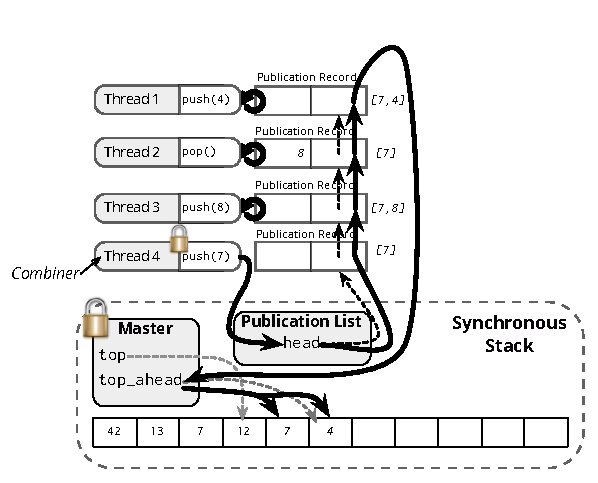
\includegraphics[width=0.5\textwidth]{figs/fc_shared_mem.pdf}
  \caption{\emph{Flat combining in shared memory.}
    To access the shared stack, each thread adds its request to the publication list (1). Thread 4 acquires the stack's lock and becomes the combiner (2), while the remaining threads spin waiting for their request to be satisfied. The combiner walks the publication list from the head, matching up Thread 3's push with Thread 2's pop on its own private stack (3). The 2 remaining pushes are added to the top of the shared stack (4). Finally, the top is updated, and Thread 4 releases the lock and continues its normal execution.
  }
  \label{fig:fc_shared_mem}
\end{figure}

One of the issues with shared data structures in a shared-memory multicore is that threads executing on different cores will force the hottest parts of the data structure to thrash between their caches. Having a single thread do all of the operations on the data structure allows it to keep everything in its cache.

% Improving locality in a shared-memory multicore is achieved by 
% Having a single thread bound to a particular core do a string of accesses trivially results in a lower cache miss rate than having multiple threads on multiple cores bring the data structure into cache each in turn.

% Careful engineering must be employed to implement a mechanism for cooperation that does not introduce the same synchronization issues as the original contended data structure.

Reduced synchronization comes from delegating work to another core.
To illustrate the issue, consider the shared synchronous queue, shown in Figure~\ref{fig:fc_shared_mem}, with pre-allocated storage and a \texttt{top} pointer protected by a lock. Without flat combining, whenever a thread attempts to push something on the stack, it must acquire the lock, put its value into the storage array, bump the top, and then release the lock. When many threads contend for the lock, all but one will fail and will have to retry. Each try forces a memory fence for consistency and consumes bandwidth, and as the number of threads increases, the fraction of successes plummets. Under flat combining, instead, threads add requests to the publication list. They each try to acquire the lock, and the one that succeeds becomes the combiner. Instead of retrying, the rest spin waiting for their request to be filled. The combiner walks the publication list, performs all of the requests, and when done, releases the lock. This has greatly reduced the synchronization on the stack's lock, but has introduced a new point of synchronization---threads must synchronize to add to the publication list. However, if a thread performs multiple operations on the stack, it can leave its publication record in the list and amortize the synchronization cost.

The above example of delegation is compelling in itself. However, the crux of the prior work is that data structure-specific optimization can be done to perform the combined operations more efficiently than separately.
As the combiner walks the publication list, it merges each non-empty publication record into a combined operation. In the case of the stack example shown in Figure~\ref{fig:fc_shared_mem}, as it walks the list, Thread 4 keeps track of the operations on its own temporary stack. When it encounters Thread 2's pop, it recognizes that it can satisfy that pop immediately with the push it just processed from Thread 3, so it fills each of their records and allows each of them to proceed. After traversing the rest of the publication list, the thread applies the combined operation to the actual data structure, in this case, the remaining two elements are pushed onto the top of the stack, and the requesting threads' records are marked as complete.
In the case of the stack, combining came in the form of matched pushes and pops, but many data structures have other ways in which operations can be matched locally.

\subsection{In Grappa}

\begin{figure*}[t]
  \centering
  \begin{subfigure}[b]{0.43\textwidth}
    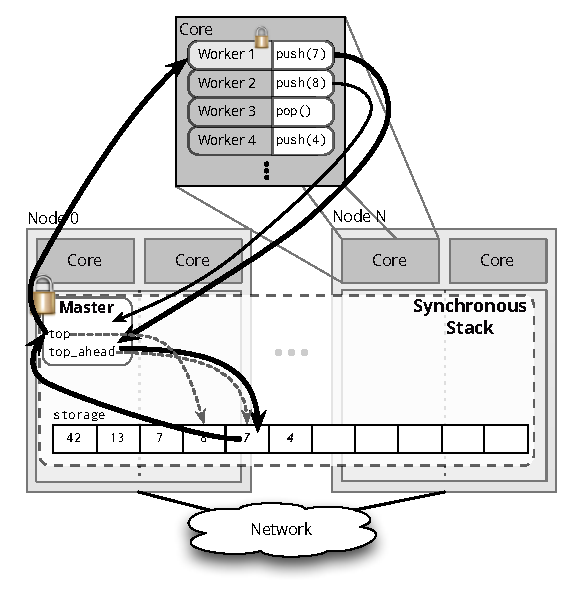
\includegraphics[width=\textwidth]{figs/stack_nofc.pdf}
    \caption{\emph{Without flat combining.}
      To do its push, Worker 1 sends a message to synchronize with the master on Core 0 (1), which sends another message to write the value to the top of the stack (2), bumps the synchronized \texttt{top} pointer (3), and finally continues. Worker 2, and all other workers on all cores accessing the stack, must block at the master and wait for Worker 1 to complete its push before doing their operations (4).
    }
    \label{fig:stacknofc}
  \end{subfigure}%
  \hspace{0.05\textwidth}
  \begin{subfigure}[b]{0.43\textwidth}
    \centering
    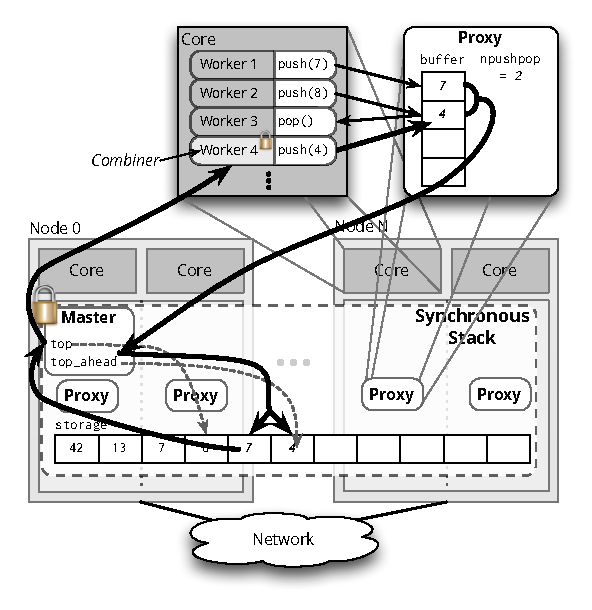
\includegraphics[width=\textwidth]{figs/stack_fc.pdf}
    \caption{\emph{Local flat combining.}
      Workers within the core add their requests to a local proxy object. Worker 3's pop matches with Worker 2's push, requiring no global communication (1). After combining locally, Worker 1 and 4's pushes remain, so Worker 4 becomes the core's combiner (2), sends a message to synchronize with the master (3), adds both new values to the global stack (4), bumps the top pointer and releases the lock on master (5), and finally wakes Worker 1 and continues (6).
    }
    \label{fig:stackfc}
  \end{subfigure}
  \caption{\emph{Global stack in Grappa} with and without \emph{flat combining}.}
  \label{fig:stack}
\end{figure*}

In a PGAS setting, and in Grappa in particular, the cost of global synchronization and the amount of concurrency is even greater than in shared memory. With thousands of workers per core, in a reasonably sized cluster there are easily millions of workers. This presents an opportunity for flat combining to pay off greatly, but also poses new challenges.

% a number of different choices are made when implementing flat combining. Because memory is physically distributed, locality must be made explicit. In addition, in Grappa there are orders of magnitude more concurrent threads (``workers'') accessing shared data structures. Typically around a thousand are needed per core to tolerate the latency of remote operations, so in a cluster of machines, there are easily millions of workers. Therefore, a different scheme for managing many threads is necessary.

To illustrate how flat combining can be applied to Grappa, we must first describe what a global data structure might look like. Figure~\ref{fig:stacknofc} shows a simple PGAS translation of the shared-memory stack from earlier. A storage array is allocated out of the global heap, so its elements are striped across all the cores in the system. One core is designated the ``master'' to enforce global synchronization, and holds the elements of the data structure that all concurrent accessors must agree on, in this case, the \texttt{top} pointer.

All tasks that want to access the global stack hold a \texttt{GlobalAddress} to the Master object. To perform an operation, the task invokes a custom delegate operation that, like the \texttt{read()} delegate described earlier, blocks the task until complete. Example code to do a \texttt{push} is shown in Figure~\ref{fig:push}, the task must send a message to the master to acquire the lock. If it succeeds, it follows the \texttt{top} pointer, writes its new value to the end of the stack, returns to bump the \texttt{top} pointer and release the lock, and finally sends a message back to wake the calling worker. All other workers performing operations block at the first message until the lock is released. Because of Grappa's user-level blocking mechanisms, blocked requests do not have to retry or busy-wait. However, all thousand workers on each core all perform this synchronization and serialize on the master core.

\paragraph{Centralized Combining.}
A first thought might be to directly apply the idea of flat combining to the serialization at the master node. The worker that acquires the lock on the master can walk through the requests of all the other workers waiting to acquire the global lock and perform combining on them. In the case of the GlobalStack, this would mean taking all of the push requests, matching them with the pops, and sending messages back to the remote workers with the results. Any leftover pushes or pops would be applied to the data structure, and another round of combining would begin. This approach, combining on the master, reduces traffic to the data structure storage, but the single ``master'' core must still process every single request. This approach will not scale when every other core can generate requests just as fast as the master can combine them.

\paragraph{Distributed Combining}
Instead of all workers on a core sending independent synchronization messages and putting the burden all on the master, what if each core did its own combining first, and synchronized with the master in bulk?
Distributing the combining to each core allows the majority of the work to be performed in parallel and without communication.
As with shared-memory combining, distributed combining improves locality, reduces the amount of global synchronization, and allows operations to be composed in data structure-specific ways for even greater performance.
% allows synchronization to happen in parallel on all the cores, 
% Flat combining in Grappa is about allowing synchronization and  distributing synchronization 
% In a way, Grappa's automatic message aggregation is already trying to reduce synchronization traffic; however, the generic mechanism for serializing and packing has a cost, and in the end, the operations must still serialize on the master.
% Flat combining is about ``teaching'' it how to more efficiently perform many operations remotely in certain special cases.

% In order for workers to cooperate locally, a local ``proxy'' object is allocated in the core-private heap. This proxy serves as the 

In distributed flat-combining, each core needs its own publication list to track all of its outstanding operations to be performed on the global data structure. In Grappa, this takes the form of a local \emph{proxy} object allocated from the core-local heap.
Conceptually, workers add their requests to the local publication list, one is chosen to do the combining, and the rest block until their request is satisfied.
However, because workers are scheduled cooperatively, each worker has atomic access to the local proxy ``for free'', so an explicit publication list is unnecessary.
Instead, each worker performs its own combining, pushing the 
, and blocks if it was unable to satisfy its request immediately. Figure~\ref{fig:stackfc} shows how in the global stack example, pushes and pops can be matched locally, avoiding global synchronization for those operations.

After all local combining has been done, one requesting worker is chosen to perform the combined operation globally. In the same figure, Worker 4 becomes the combiner and performs much the same synchronization as in the un-combined case, but is able to push multiple elements with one synchronization. As in the uncombined case, the global lock must still be acquired, and concurrent combined requests must still block and serialize on the master, though a technique later will describe how flat combining can be applied here, too. Combining in this way allows synchronization to be distributed and performed in parallel, coarsening the granularity of the actual global synchronization and reducing the amount of serialization that occurs.

% In most cases, this means communicating with whichever core holds the ``lock-protected'' field that maintains sequential consistency. In the case of a global stack, this is the ``master'' \emph{top} pointer which must be incremented on pushes and decremented on pops. On the core where global synchronization is occurring, there must be synchronization between the multiple synchronization requests arriving from other cores.

% At this point we have traded off one remote synchronization per operation for an additional local synchronization per operation and some number fewer remote synchronizations (depending on the amount of combining that occurs). This would likely result in a net benefit due to local synchronization being inherently cheaper. However, because of the way the Grappa runtime schedules computation, it is actually possible to get the correct mutual exclusion/atomicity without any additional synchronization overhead.

% By design, each core in Grappa operates independently of the other cores. Workers are scheduled cooperatively, so each worker can assume atomicity until it performs an operation that yields to the scheduler, such as a remote call. Therefore workers within a core can cooperate without any explicit synchronization operations requiring memory fences. This allows them to publish requests to the local proxy very inexpensively, eliminating the need for a complex synchronization-amortizing queue. This has the added benefit that there will be no unused publication records, which could have become a problem with thousands of workers. Further, remote operations are processed through the same cooperative-multithreading scheduler on the remote side, so combined operations are trivially serialized and atomic.

\paragraph{Sequential Consistency}
The sequential consistency guarantee is that within a task, operations will be in task order, so to enforce ordering between operations in different tasks, one task must perform an operation that another one can observe. An example is shown in Figure~\ref{fig:sync}.\TODO{make sync example}
The Grappa memory model is in the style of the C++ memory model~\cite{boehm:drf0,N2480,N2800} memory model (guaranteeing sequential consistency for data-race free programs). Being conservative, delegate operations block the calling worker until they have completed globally, ensuring they can be used for synchronization. As such, delegate operations within a task are guaranteed to be globally visible in program order.
Because it is not immediately obvious that this distributed version of flat combining preserves sequential consistency, here we will make arguments for why it does.

% \begin{itemize}
%   \item Block the calling worker until the operation is guaranteed to have a valid global order.
%   \item Local combining must not allow workers to observe a different order than is committed globally.
% \end{itemize}
To preserve sequentially-consistent semantics for flat-combined operations, they must obey a consistent global order.
To start with, local combined operations must have a serializable order among each other; this is unchanged from shared-memory flat-combining, and is trivially true due to the atomicity enabled by cooperative multithreading.
When combined operations are applied globally, they are serialized at a particular core that owns the synchronization (the ``master'' core for the Queue and Stack, or the corresponding hash cell for the Set and Map). The global order, then, is essentially the concatenation of the cores' sequential orders.
For this ``concatenation'' to be valid, the order observed by workers during local combining must be the same as what can be observed globally as operations are committed.

In the case of the Stack and Queue, this guarantee comes from applying a batch of push or pop operations atomically in a contiguous block on the global data structure. The second level of combining at the master preserves this as well by only allowing updates to proceed when they will not conflict and blocking all of them until they have completed.
Matching pushes and pops locally is one exception to the rule that operations must block until globally committed. Because a pop ``destroys'' the corresponding push, these operations together are independent of all others and can conceptually be placed anywhere in a total global ordering, so they can be safely matched locally.

The correctness of combining set and map operations is more nuanced.
Insert and lookup operations performed by different tasks are inherently unordered unless synchronized externally.
Therefore, a batch of these operations can be committed globally in parallel.
If an insert finds that its key is already in the combiner, it does not need to send its own message. However, it must still block until that insert is done, otherwise it may assume that the key has been inserted and perform some other operation that requires the insert to have happened.
In the same way, lookups can piggy-back on other lookups of the same key.
It is tempting to allow a lookup to be satisfied locally by inspecting the keys to be inserted.
However, this allows the local order in which keys were inserted to be observed.
If this is allowed, then that same order must be respected globally, forcing each batch to ensure atomicity from all other cores' batches. This is prohibitively expensive, so a cheaper solution is chosen: lookups must get their values from the global data structure, but can be performed in parallel in the same way as inserts.

% (wrong!) A lookup can be satisfied locally provided that the insert it relies on is guaranteed to eventually be committed globally. This allows the task to continue. If it does another lookup to a different key that is satisfied locally, then that task has observed one particular ordering of the two inserts. When those inserts commit globally, they will proceed in parallel to their respective hashed locations. Another task could 

% The combining operations that are performed locally among requests on a single core must preserve the illusion of sequential order; this is unchanged from shared-memory flat-combining. When combined operations are applied globally, they are serialized at the ``master'' core for a given synchronization context. The global order is essentially the concatenation of each core's batch of serialized accesses.
% In the case where operations are satisfied locally (by matching up with other local operations), by definition these must be independent of other operations, so they can conceptually be placed anywhere in the global ordering (or even ignored completely in the global ordering).

% In the spirit of the Data-Race-Free-0 Model (guaranteeing sequential consistency for data-race free programs), operations on the global data structure are considered to be made atomic by a conceptual global ``lock'' on the data structure. 

These requirements only guarantee sequential consistency for a data structure in isolation. Atomicity and data race freedom in the case of multiple data structures must be guaranteed externally, just as in any multithreaded shared-memory program.

\section{Grappa FC Framework}
% One of the strengths of flat combining is that the same combining mechanism can be applied in multiple data structures. Each structure must only specify how its operations compose.
% Many different data structures can integrate flat combining into their operation using the same delegation mechanism, making it easier to implement concurrent data structures.
In order to leverage the flat-combining paradigm in Grappa, we implemented a generic framework which can be used to improve performance for a number of global data structures. The FC framework handles the common problems of managing the combiners, handling worker wake-ups, and maintaining progress. When hooking into the framework, each data structure implementation need only define how to combine operations and globally commit them.

% As discussed before, Grappa's distributed combining takes a different approach to expressing how operation locally  flat combining design takes a different approach to performing 
The Grappa FC framework takes a different approach than the original flat-combining work for expressing how operations combine. As mentioned before, the local ``publication list'' is trivial to access atomically in Grappa due to workers being cooperatively scheduled.
Instead, in the Grappa FC Framework, a \emph{proxy} object is instantiated ahead of time on each core and each worker merges its update into that structure before blocking or becoming the combiner.
% In the original work, an explicit publication list is built up, and when the combiner scans over the list, it has a structure that it uses to accumulate requests in a logical way. In the case of the stack, for instance, it is a thread-local stack, which it can use to immediately match up pushes and pops. In the Grappa implementation, each worker's actions are atomic anyway, so rather than creating an explicit request list, the combiner object (or \emph{proxy}) is instantiated ahead of time for the data structure, and each worker does its own local combining into that structure before blocking. This reduces the space blowout of a large dynamically-sized publication list (with associated caching issues), and does not overly affect the expression of combining.
In this style, each global data structure must define the following:
\begin{enumerate}
  \item A local \emph{proxy} data structure for tracking updates to the global structure.
  \item \emph{Combining methods} that operate on the local proxy.
  \item A \emph{sync} method that globally commits the proxy's state.
\end{enumerate}
An example proxy declaration for the GlobalStack is shown in Figure~\ref{fig:proxy}.

\begin{figure}[t]
\centering
\begin{lstlisting}[style=grappa]
class GlobalStack {
  GlobalAddress<T> top;
  Grappa::Mutex lock;
};

void push(GlobalAddress<GlobalStack> stack, T e) {
  // perform operation on the stack's master core
  delegate::call(stack.core(), [stack,e]{
    // force other operations to wait
    stack->lock.acquire();
    // do remote write to the top of the stack
    // (so other workers may interleave)
    delegate::write(stack->top, e);
    // bump the top pointer
    stack->top++;
    stack->lock.release();
  }); // blocks until response arrives
}\end{lstlisting}
\caption{Snippet of code for pushing to a global stack (without flat combining).}
\label{fig:push}
\end{figure}

\begin{figure}[t]
\centering
\begin{lstlisting}[style=grappa]
class GlobalStackProxy : Grappa::FCProxy {
  // pointer to data structure master
  GlobalAddress<GlobalStack> master;
  
  // local state for tracking pushes and pops
  T  pushed_values[1024];
  T* popped_results[1024];
  int npush, npop;

  // Combining Methods 
  // (either match locally or block for results)
  void push(T val);
  T pop();
  
  // Global sync (called by FC framework)
  void sync() override {
    if (npush > 0) {
      // on master, acquire lock and return GlobalAddress to the top of the stack
      auto top = delegate::call(master.core(),[=]{
        master->lock.acquire();
        return master->top;
      });
      // copy values to top of stack
      Grappa::memcpy(top, pushed_values, npush);
      // release lock at the master core
      delegate::call(master.core(),[master,npush]{
        master->top += npush;
        master->lock.release();
      });
    } else if (npop > 0) {} //...elided for space
  }
};
\end{lstlisting}
\caption{Snippet of the Proxy object for the GlobalStack. The code to synchronize pushes should resemble that from Figure~\ref{fig:push} but for multiple elements.}
\label{fig:proxy}
\end{figure}

With this data structure-specific proxy object, the FC framework does the bookkeeping to block and wake Workers, deliver results, manage when to synchronize, and choose the combiner.
The FC framework is responsible for ensuring that all of the combined operations eventually get committed. There are a number of ways progress could be guaranteed, but one of the simplest is to ensure that as long as there are any outstanding requests, at least one worker is committing a combined operation.
When that combined operation finishes, if there are still outstanding requests that have built up in the meantime, another blocked worker is chosen to do another combined synchronization.

One could imagine other synchronization policies that would ensure progress but allow more combining to occur before synchronizing. For instance, local combining could continue until all workers are blocked. However, this would require the flat-combining framework to track the activity of the workers on a core, and additionally would add latency unless the system saved enough active workers to tolerate the latency of the global commit action. As it is, the one-in-flight policy implemented performs well, and does not require any coupling with the Grappa scheduler. Exploration of other policies is left for future work.

While a combining operation is in flight, new requests are likely to continue to accumulate. The framework transparently wraps the proxy object so that when it starts a sync on one, it can direct requests to a fresh combiner. It is important to note that combiners must start out fresh each time---it would be unsound for them to ``remember'' the previous updates and attempt to combine locally with them.

% The flat combining framework transparently wraps the \emph{proxy} object. Behind this layer of indirection, it manages multiple copies of the proxy so that, as discussed above, there is always at least one being committed and one to receive additional combining operations.

% explain simple non-combined global data structures in Grappa section...

\subsection{Global Stack and Queue}
Figure~\ref{fig:proxy} shows an excerpt from the definition of the proxy object for the Grappa GlobalStack. The proxy tracks pushes locally in the \texttt{pushed\_values} array. When \texttt{pop()} is called, if there are pushes in the local array, it immediately takes the value and wakes the last worker to push. Otherwise, it adds a pointer to a location on its stack where the \texttt{sync} operation, will eventually write the result. Because of local matching, when a Stack proxy is synchronized, it will have either all pops or all pushes, which makes the implementation of sync straightforward. Note that the operation to synchronize a batch of pushes looks almost identical to the code to do a single push from Figure~\ref{fig:push}.

The GlobalQueue has nearly the same implementation as the stack, but is unable to match locally, so \texttt{sync} first does the pushes, then does the pops.

\subsection{Global Set, and Map}
The Grappa GlobalSet uses a simple chaining design, implemented with a global array of cells (allocated from the global heap), which are partitioned evenly among all the cores, and indexed with a globally-agreed hash function. Our flat-combining version supports both \texttt{insert} and \texttt{lookup}. To track all of the keys waiting to be inserted, we use the hash set implementation from the C++11 standard library (\texttt{std::unordered\_set}). Similar to the case with pops, for lookups, we must keep track of pointers for where to put the results of lookup operations, which the proxy does with a hash map (again from the C++ standard library) from keys to a list of pointers. As discussed in Section~\ref{sec:sc}, matching lookups with inserts locally would force a particular sequential order, so instead we only allow matching inserts with inserts and lookups with lookups. This allows \texttt{sync} to simply issue all of the inserts and lookups in parallel and block until all have completed.

Our implementation of the GlobalMap matches that of the Set, but of course stores values of a given type. This does not change the requirements of the proxy except that the return values of lookups must be a copy of the value rather than just a boolean.

